\documentclass[a4paper,AutoFakeBold,oneside,12pt]{book}
\usepackage{BUPTthesisbachelor}
\usepackage{setspace}

%\lstdefinestyle{sharpc}{language=[Sharp]C, frame=lrtb, rulecolor=\color{blue!80!black}}


%%%%%%%%%%%%%%%%%%%%%%%%% Begin Documents %%%%%%%%%%%%%%%%%%%%%%%%%%
\begin{document}

% 封面

\includepdf[pages=-]{docs/cover.pdf}  
\newpage

% 任务书
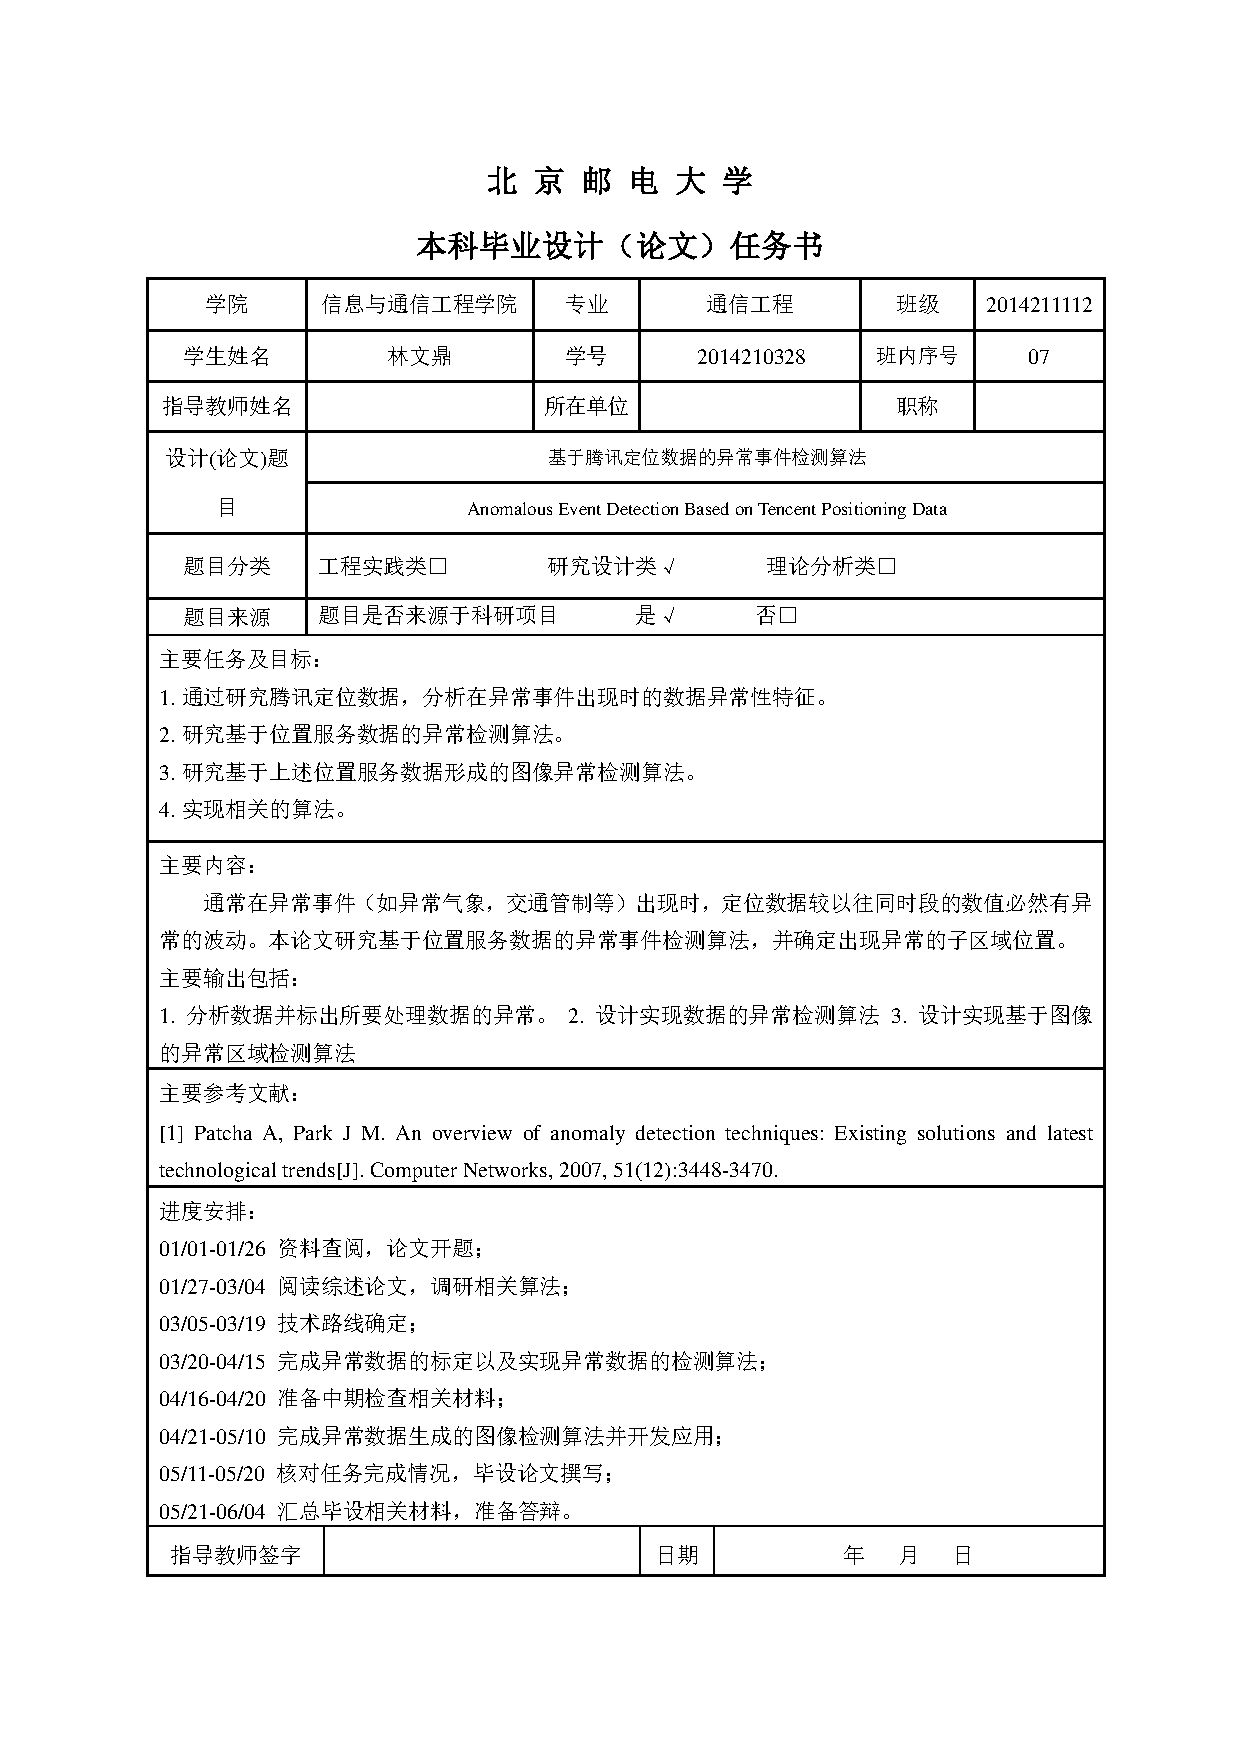
\includepdf[pages=-]{docs/task.pdf}  
\newpage

% 成绩评定表
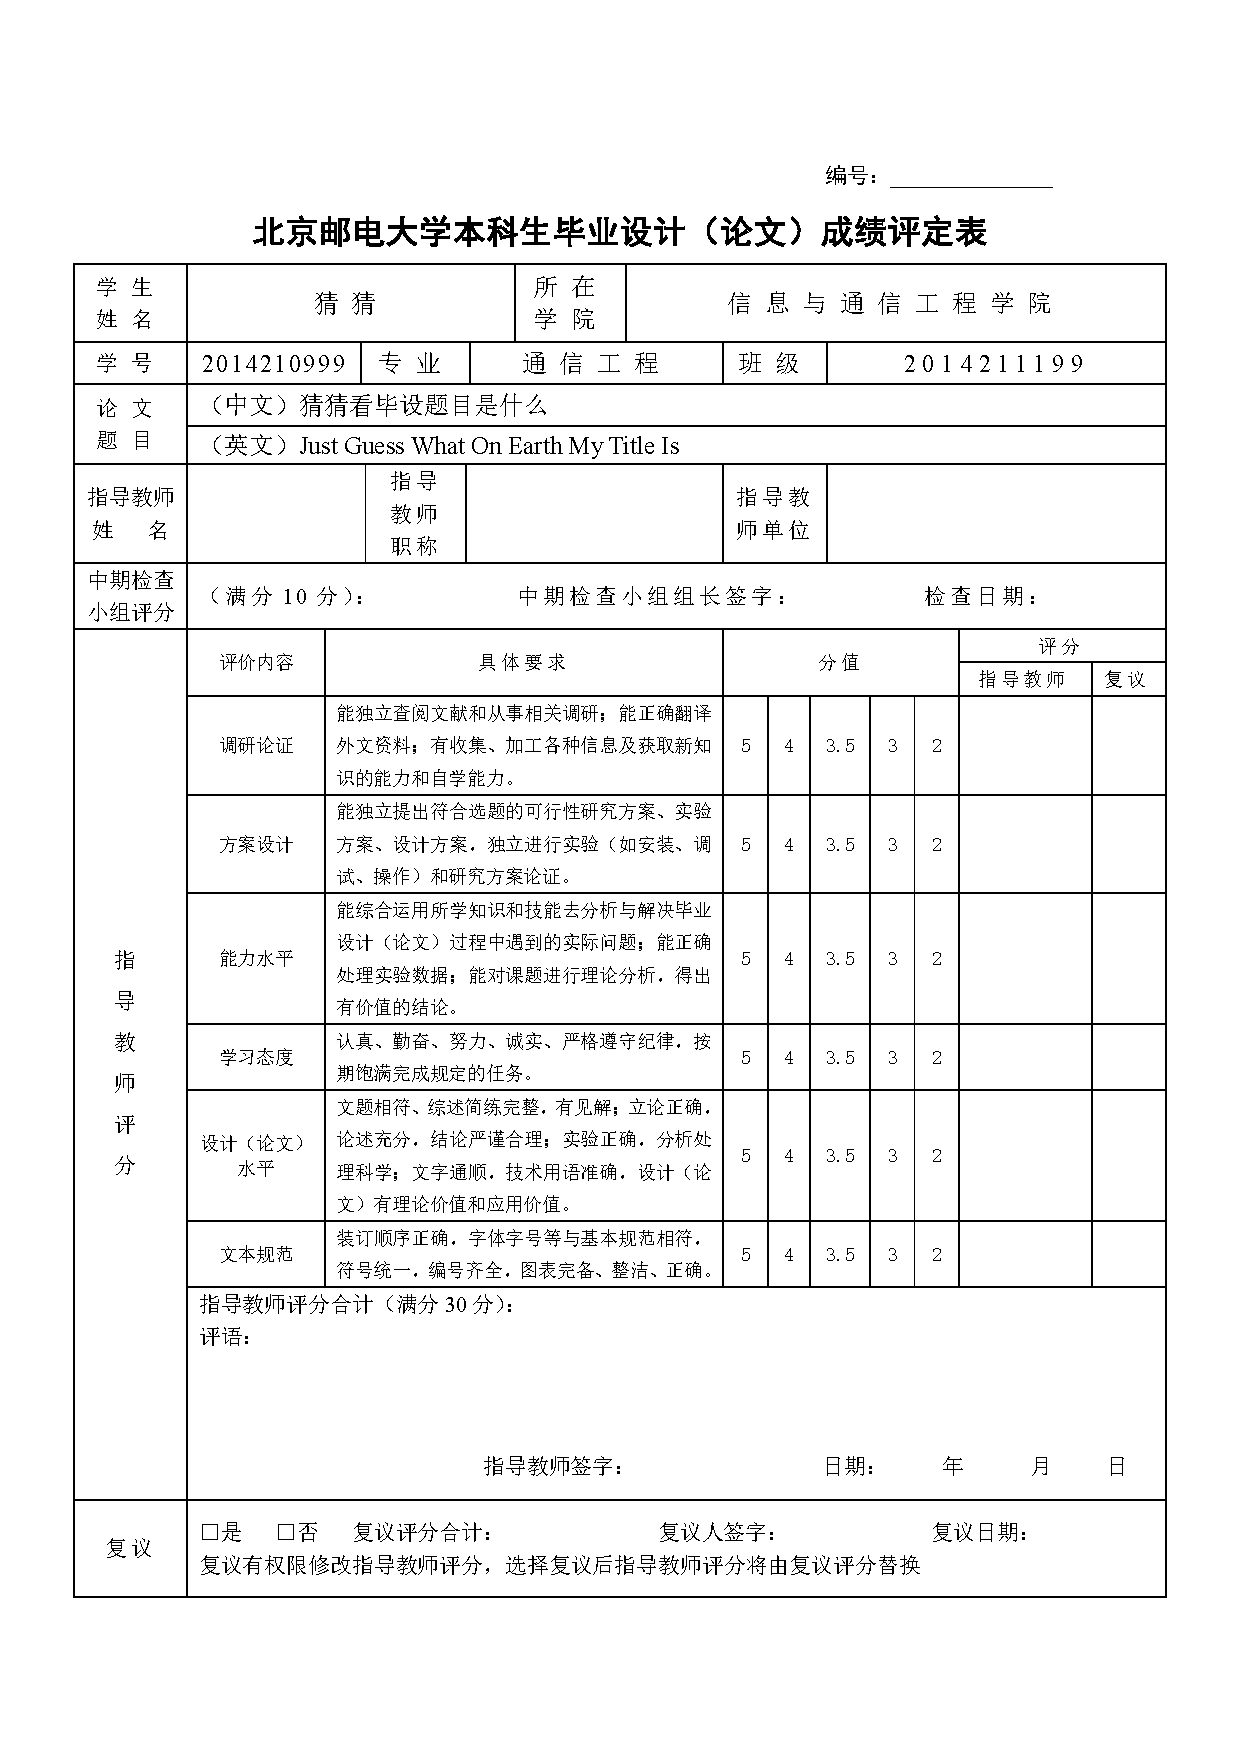
\includepdf[pages=-]{docs/scoreTable.pdf}  
\newpage

% 诚信声明

\includepdf[pages=-]{docs/statement.pdf} 
\newpage

%%%%%%%%%%%%%%%%%%%%%%%%%%%%%%%%%%%%%%%%%%%%%%%%%%%%%%%%%%%%%%%%%%%%
%                                                                  %
%   Copyright (c) 2010 - 2011 Caspar Zhang <casparant@gmail.com>   %
%                                                                  %
%   This copyrighted material is made available to anyone wishing  %
%   to use, modify, copy, or redistribute it subject to the terms  %
%   and conditions of the GNU General Public License version 2.    %
%                                                                  %
%   This program is distributed in the hope that it will be        %
%   useful, but WITHOUT ANY WARRANTY; without even the implied     %
%   warranty of MERCHANTABILITY or FITNESS FOR A PARTICULAR        %
%   PURPOSE. See the GNU General Public License for more details.  %
%                                                                  %
%   You should have received a copy of the GNU General Public      %
%   License along with this program; if not, write to the Free     %
%   Software Foundation, Inc., 51 Franklin Street, Fifth Floor,    %
%   Boston, MA 02110-1301, USA.                                    %
%                                                                  %
%%%%%%%%%%%%%%%%%%%%%%%%%%%%%%%%%%%%%%%%%%%%%%%%%%%%%%%%%%%%%%%%%%%%

% 你只需要修改下面几行就可以完成大部分内容的填写,
% 这要求你具有一定的LaTeX基础,但是如果你足够聪明,
% 不具有LaTeX基础也可以完成。

% 论文中文题目
\def\thesistitle{基于腾讯定位数据的异常事件检测算法}

% 论文英文题目
\def\thesistitleen{Anomalous Event Detection Based on Tencent Positioning Data}

% Thank Words
\def\thankwords{

本次毕业设计是在***老师的悉心指导下完成的。从课题的选择、设计到论文的撰写一直到最后论文的定稿,期间遇到很多问题,都得到了***老师全力细心的指导。在此,向***老师表示衷心的感谢!

感谢信息与通信工程学院所有老师多年来对我的培养、帮助,使本人在本科学习中不仅学到了必备的专业知识技能和思考解决问题的方法,还学到了严谨治学的科研精神和积极进取的人生态度。

同时,感谢信息与通信工程学院的所有同学,给我创造了一个团结进取,充满温暖,充满爱的大集体,使我快乐而且充实地度过了人生中最美好的大学时光。

感谢提供此论文模板的开源项目https://github.com/sqyx008/BUPTBachelorThesis


	
}
    % Main items 
%%%%%%%%%%%%%%%%%%%%%%%%%%%%%%%%%%%%%%%%%%%%%%%%%%%%%%%%%%%%%%%%%%%%
%                                                                  %
%   Copyright (c) 2010 - 2011 Caspar Zhang <casparant@gmail.com>   %
%                                                                  %
%   This copyrighted material is made available to anyone wishing  %
%   to use, modify, copy, or redistribute it subject to the terms  %
%   and conditions of the GNU General Public License version 2.    %
%                                                                  %
%   This program is distributed in the hope that it will be        %
%   useful, but WITHOUT ANY WARRANTY; without even the implied     %
%   warranty of MERCHANTABILITY or FITNESS FOR A PARTICULAR        %
%   PURPOSE. See the GNU General Public License for more details.  %
%                                                                  %
%   You should have received a copy of the GNU General Public      %
%   License along with this program; if not, write to the Free     %
%   Software Foundation, Inc., 51 Franklin Street, Fifth Floor,    %
%   Boston, MA 02110-1301, USA.                                    %
%                                                                  %
%%%%%%%%%%%%%%%%%%%%%%%%%%%%%%%%%%%%%%%%%%%%%%%%%%%%%%%%%%%%%%%%%%%%

% 你只需要修改下面内容就可以完成中英文摘要,
% 这要求你具有一定的LaTeX基础,但是还是那句话,
% 如果你足够聪明,不具有LaTeX基础也可以完成。

% 中文摘要
\def\abstractzh{
%从这里开始写你的摘要,分段需要空一行。

通过终端设备采集的定位数据的大小反映了这个区域的人口密度特征,而通过长时记录所得到的时序定位数据更能反映密度的变化特征。人口密度的变化特征通常在时间上符合一个规律,而在某些时刻由于例如自然灾害的原因会导致该地的定位数据异常,检出这种异常能够使有关部门做好应急响应。本文基于腾讯定位数据,对确定区域的定位数据进行异常检测,研究相关的算法,并尝试确定出现异常的子区域位置。

针对以上目的,本文对给定的定位数据进行了分析及预处理,采用了基于差分、小波、极大似然估计、局部异常因子的几种曲线异常检测算法对诸如台风过境的区域全天性异常进行了检测,然后使用了非线性自回归网络基于过往时刻数据对当前时刻定位值进行曲线预测,检测了局部时刻的异常值,最后运用了帧间差分法,针对检测出的异常出现时刻使用了不同大小的滑动窗计算区域定位数据变化平均值来确定异常发生的核心子区域位置。

在基于给定的腾讯定位数据基础上,仿真结果表明:使用了曲线异常检测与预测的方法可检出区域性的整天性时段与局部性时刻异常,而通过相邻帧间差分法与滑动窗相结合能够将造成异常的主要区域检出。
%摘要结束
}

% 中文关键字 
% TODO: 改成可变长度的
\def\abszhkeyone{定位数据}
\def\abszhkeytwo{异常检测}
\def\abszhkeythree{曲线分析}

% ABSTRACT
\def\abstracten{
%Your abstract here, to make a new paragraph, give an extra blank line please.
The size of the positioning data collected by the terminal equipment reflects the population density characteristics of this area, and the time-series positioning data obtained by the long-term recording can better reflect the population density variation characteristics of the area. The characteristics of changes in population density usually conform to a rule in time. At some moments, for example, due to natural disasters, the location data of the area may be abnormal. The detection of such anomaly can enable the relevant departments to make an emergency response. In this paper, based on Tencent positioning data, we try to detect the anomaly of positioning data in a certain area, study relevant algorithms, and search the location of an abnormal sub-area in there.

For the above purposes, this paper analyzes and preprocesses the given positioning data, and adopts several curve anomaly detection algorithms based on difference, wavelet, maximum likelihood estimation, and local outlier factors for regional whole day anomaly such as typhoon crossing. Then a non-linear autoregressive network was used to curve the current local time value based on past time data to detect the hour anomaly. Finally, the inter-frame difference method was used to detect the occurrence area of the anomaly. Different sliding window sizes are used to calculate the average regional positioning data change values to determine the location of the core sub-area where the anomaly occurs.

Based on the given Tencent positioning data, the simulation results show that using the method of curve anomaly detection and prediction can detect regional all-day and local-time anomalies, and through adjacent inter-frame difference method and sliding The combination of windows can detect the main area causing the anomaly.

%Abstract done
}

% Key Words 
% TODO: 改成可变长度的
\def\absenkeyone{positioning data}
\def\absenkeytwo{anomaly detection}
\def\absenkeythree{curve analysis}



  % Abstract
\frontmatter\tableofcontents % Content

% 正文
\newpage\mainmatter
\fancypagestyle{plain}{\pagestyle{fancy}} % Add head to new chapter
\pagestyle{fancy} % Head and foot
%\let\cleardoublepagebak=\cleardoublepage
%\let\cleardoublepage\relax % Make new chapter stay on old page

%%%%%%%%%%%%%%%%%%%%%%%%%%%%% Main Area %%%%%%%%%%%%%%%%%%%%%%%%%%%%

\chapter{绪论}

% 如果你的项目来源于科研项目,可以使用以下指令插入无编号脚注于正文第一页
%\blfootnote{本项目来源于科研项目“基于\LaTeX{}的本科毕业设计”,项目编号1124}

本章主要介绍了定位数据的异常事件检测的课题背景及其研究意义,其次介绍了异常检测这一领域的基本概念及常用算法分类,最后对论文的主要研究工作进行了总结并阐述了本文的行文章节安排。

\section{课题背景}

随着GPS定位,传感器网络和高速无线通信等技术的日益发展,越来越多的终端定位数据被收集和保存在应用服务器,它们是各地人口密度的一个衡量依据。除了定位数据本身所体现的人口密度空间特征,在相同的空间位置不同的时间点上进行记录还可以得到定位数据的人口密度时序特征。而通过分析某片区域上的时序定位数据,可以得到该区域上人口密度的变化特征,例如从北京市每日的滴滴打车的定位数据可以明显地总结出以下特征:滴滴车辆在早高峰时将大量住在郊区的人群运送至各大工作区(例如中关村和国贸区域),而在晚高峰时它们又将人群从工作区运送回家,如下图所示。这种区域性的时序定位数据反应出了北京市的日人口密度变化特征。

	在这种区域性的时间序列中,也会在某些时间点上出现这样的观测点,它们较以往同时段的数据,例如某个星期天与前几周的星期天来说,会有一个明显的波动,这就是时序数据点中的异常值。分析这些异常点也是一个很重要的课题,通常对于区域性时序特征模型的建立,这些异常点是应当被剔除的噪声,它们会对模型的预测功能产生极大的阻碍。但同时异常点也可以作为一些突发事件(如异常气象,交通管制等)的判断因素,在异常事件发生时,区域的时序定位数据会在某一个时间间隔中出现较大的落差,即异常波动,通过异常检测算法将上述波动检出并分析,可以使有关部门察觉到异常状况的发生并及时做好应急响应。


\section{异常检测研究现状}

\subsection{基本概念与挑战}

“异常”是指数据特征不符合该特征一般所隶属区间的现象。寻找异常是一个非常困难的课题,其难点主要来源于以下两个角度:首先,“异常”通常情况下只是一个定性的概念,偏离正常数据多少可以被界定为异常没有一个定量的比例数值,那么对于那些处于异常非异常边界线附近的异常数据来说,完全可以把边界线略微移动,使其能被归类为正常的数据;再者,用于划定数据特征正常区间的正常样本中有时也会存在异常数据,导致划定边界线偏差或是训练出的预测模型不准确。同时,考虑到正常的数据量远大于异常数据,使用机器学习的方法进行训练时很容易使网络结构偏向于正常数据的分布,即过拟合导致无法检测出异常。
为了便于分析,异常也有多种分类:通常情况下直观理解的异常指的是点异常,其含义是多个数据实体中,如果存在一个实体对于其他实体来说有极大的偏差,那么这个实体数据所对应的特征就表明一种点异常。而另外一种异常被称为环境异常,它与点异常中的异常概念是一样的,表征的是一个数据实体在特定环境中的异常,存在某种限定条件。这种异常类型的数据实体有两部分组成:环境属性与行为属性。环境属性表征了数据实体所处在的环境,例如时间序列数据的时间点,空间数据的地理坐标;行为属性表征了在上述特定环境属性下区分数据实体的属性,类似于地理数据的某地降雨量,行为属性即固定了环境属性后的数据特征,例如已知某地理坐标上的定位数据量。在本课题中,数据属于时序性的定位数据,而其中的异常是一种环境异常。环境属性即是时空坐标与地理坐标,行为属性是在某时间点上某地理坐标下的定位终端数量。

\subsection{异常检测算法分类}

异常检测是找出数据特征严重不同于预期对象的一个检测过程。传统检测异常的方法分为以下几类:基于分类的异常检测方法,基于最近邻的异常检测方法,基于聚类的异常检测方法,基于统计的异常检测方法。
	1. 基于分类的异常检测方法:分类是一种从一组已做好标注的数据实例(训练)中学习模型(分类器),然后使用学习模型(测试)将测试实例分类到其中一个类中的方法。基于分类的异常检测算法以类似的两阶段方式生成一个分类模型从而判断数据的特征是否异常:在训练阶段通过使用已进行标记的样本来训练分类器的模型和参数;测试阶段使用分类器将测试实例分类为正常或异常。基于分类的异常检测算法基于以下假设下实现:在给定的数据特征空间中学习可以区分正常类和异常类的分类器是可行的。
	2. 基于最近邻的异常检测方法:近邻分析的概念已用于多种异常检测算法,这些算法都基于以下关键假设:正常的数据实例发生在密集的邻域中,而异常发生在离它们最近的邻居很远的地方。最近邻的异常检测算法需要两个数据实例之间所定义的距离或相似度衡量,而这些距离又针对不同类别的属性有不同的衡量标准。对于连续的属性,欧几里得距离的效果优秀,可以表征出两个数据间的联系性,但在不同情况下也可以使用其他方法计算。对于分类属性,通常使用简单的匹配系数,但也可以使用更复杂的距离度量。对于多变量数据实例,通常为每个属性计算距离或相似度,然后进行合并。
	3. 基于聚类的异常检测方法:聚类用于将类似的数据实例分组到集群中。尽管聚类是无监督式学习,但聚类在半监督式学习中的应用也被最近探讨。尽管聚类和异常检测看起来彼此根本不同,但是已经有几种基于聚类方法被应用于异常检测:

第一类基于聚类的算法依赖于以下假设:普通数据实例属于数据中的一个集群,而异常不属于任何集群。基于此假设的技术将已知的基于聚类的算法应用于数据集,并将任何不属于任何聚类的数据实例声明为异常。
第二类基于聚类的技术依赖于以下假设:正常的数据实例靠近它们最接近的集群质心,而异常距离它们最近的集群质心很远。基于这种假设的技术由两个步骤组成。在第一步中,数据使用聚类算法进行聚类。 在第二步中,对于每个数据实例,计算它到最近的集群质心的距离作为其异常分数。
如果数据中的异常自身形成聚类,这些技术将无法检测到这种异常。为了解决这个问题,已经提出了第三类基于聚类的算法,它依赖于以下假设:普通数据实例属于大型且密集的集群,而异常集群属于小型集群或稀疏集群。基于此假设的技术将属于大小和/或密度低于阈值的集群的实例声明为异常。请注意,如果数据中的异常自身形成集群,则这些技术将无法检测到这种异常。

4. 基于统计的方法:统计异常检测技术基于以下关键假设:正态数据实例出现在随机模型的高概率区域,而异常发生在随机模型的低概率区域。统计技术将一个统计模型(通常用于正常行为)与给定数据相匹配,然后应用统计推断测试来确定一个看不见的实例是否与该模型相符。基于应用的测试统计信息从学习模型中生成概率较低的实例被声明为异常。

\section{论文主要工作}

本文基于以上课题背景以及研究现状,基于腾讯地图所提供的时序定位终端地图数据,在已知某一天为异常天(台风过境)的前提下,研究并实现检测出该天为异常天的算法,同时实现了根据现有的前几日时序定位数据预测当日定位数据的生成模型,最后使用图像处理的方法,根据异常时间点检测结果识别出造成异常的主要区域。我们对这几块内容进行了讨论并将上述成果以简易MATLAB应用的形式输出。具体实现内容包含以下几部分:
	1.	 对腾讯定位数据进行解析及预处理。首先,由于研究的异常为台风过境时某区域的定位数异常,将定位数据的区域统一标定在该地域的经纬度;其次,对定位数据进一步作图分析,观察在相同位置处定位终端数量一天内的变化、每天同时段的变化,确定了分析上述异常的策略;最后,根据数据特点进行预处理便于分析。
	2.	 对经过处理后的数据采取曲线分析的形式进行天异常检测。采用了诸如小波变换,极大似然估计法,差分分析法等传统方法以及一些混合改进算法,对这些算法的效果进行对比分析,根据数据结果总结了在该定位数据下哪一种算法实现结果最佳。
	3.	 根据处理后的数据以及曲线异常检测的结论,设计并实现曲线预测模型。采用动态神经网络使用现有数据进行训练,并使用后续补充的数据进行验证,证明了采用预测模型的方法可以有效避免只分析单异常天的弊端,以及拓展了异常检测的时间精度。
	4.	 在前述几章中数据的处理及算法的设计基础上,异常天能够被成功检出,并且根据现有的前序时序数据可以判断更高精度的实时异常。在这一章中我们使用图像分析中的帧间差分法以及滑动窗的方法确定造成整体异常的区域。
	5.	 将上述功能整合到简易MATLAB应用中。

\section{论文章节安排}

	第一章 绪论。本章主要介绍了定位数据的异常事件检测的课题背景及其研究意义,其次介绍了异常检测这一领域的基本概念及常用算法分类,最后对论文的主要研究工作进行了总结并阐述了本文的行文章节安排。
	第二章 异常检测算法基础。本章主要介绍了异常检测的算法理论基础,涵盖后续几章所用的主要算法的一些理论背景,包括了极大似然估计,小波变换,神经网络等相关概念。
	第三章 定位数据。本章主要介绍了本课题所研究的腾讯定位数据的形式,并在MATLAB中作图分析其数据特征,包含时序特征及地理特征,最后根据分析结果讨论如何进行检测。
	第四章 基于曲线分析的定位数据异常检测。 本章主要基于第三章数据分析的结果从曲线的角度对数据进行异常检测,研究了在数据中找出异常的方法。使用了例如小波变换、极大似然估计和邻域的方法进行了分析,并对这些方法的效果进行了讨论。
	第五章 定位数据的预测分析。 本章主要对异常检测的另一种思路进行了探讨,即实时判断数据是否异常的检测方法。采用了动态神经网络训练时序数据预测模型,并根据预测与实际值比对的结果对异常检测的效果进行了分析。
	第六章 基于区域的定位数据异常检测。 本章基于前述两章的异常检测结果,检测造成异常的重点区域。采用了图像分析的策略,例如帧间差分法,将异常的核心区域变化特征凸显并使用滑动窗标记。
	第七章 总结与展望。本章主要对基于腾讯定位数据的异常检测算法进行分析总结,针对实验结果进行分析,获得本文方法存在的缺点并且提出解决存在问题的有效方法,提高异常检测的准确率和平台使用的有效性。



\chapter{异常检测算法基础}
本章主要介绍了本课题所研究的异常检测的算法基础,因为在后续几章中要根据本课题所研究的数据对象对算法进行改写,所以在本章中主要介绍理论基础,后续章节中再具体阐述实际应用策略。


\section{时序曲线离群点检测}
\subsection{极大似然估计}
极大似然估计一种反推样本模型参数的统计方法。其通过对已知的样本信息建模,在数据符合某种特定分布下对分布中的参数进行似然估计。当给定了足够多的观测数据情况下,利用这些大量的试验结果去计算参数值为多少才最有可能导致这样的实验样本结果,即已经知道骰子的大量独立投掷结果去计算扔到骰子各个面的概率参数值。例如已知数据集的采样是独立且为正态分布时,我们可以使用极大似然估计法求出参数μ和σ的值。设已知样本集为:
	似然函数(Link函数):
	θ值是未知的参数值,我们要对其进行估计,如果它的值可以在范围内使前述似然函数的值最大,则它是造成这样的试验样本的最大可能值,即是θ参数的最大似然估计量。它是样本集的函数,记作:
	已知试验样本服从独立的正态分布 ,则试验样本的似然函数如下式所示:
	它的对数:
	求导,得方程组:
	联合解得:
	在上述条件下,似然方程存在唯一的解:它必须是最大点,因为它是一个非负函数何时或何时。因此u和极大似然估计是。
\subsection{离散序列小波变换}
时序信号或序列存在大量信息,但是仅仅从时序的角度去分析信号会损失大量有效信息。Fourier变换提供了一种变换域分析的方法,它利用大量的三角基去构造信号,从频域的角度对信号分析,得出更多信号的信息。美中不足的是,Fourier变换只能反映信号的频域特征,即将整个时序信号的频域分量提出,而不能反映各个时间点上的频域特征。短时Fourier变换(STFT)对此进行了改进,使用了定长的窗口对信号的时间进行了限制从而可以将每个短时进行Fourier频谱分析,最终得到时间轴上的频域特征。
	小波变换是对短时Fourier变换的进一步改进,与后者不同的是,小波并非使用固定的窗口去限定时间,而是使用随时间变化的窗口-小波基去构造短时的Fourier分析。它可以有效地改善STFT中对于随时间信号幅度变化很不均匀的信号无法妥善处理的缺点。
	小波变换和Fourier变换类似,都有应用于连续信号及离散信号的分析方法。本课题所研究的时序数据应当使用离散序列小波变换,它基于Mallat算法将时序信号按照低频信号与高频信号进行逐层分解,每一层的低频信号被继续分解为低高频信号,以此类推,具体的分解关系如下图所示:
	时序离散序列的初始向量系数x在经过一层分解后得到高频部分D1(系数的高频部分)与低频部分A1(系数的低频部分),这两个分量是原始信号分别经过高通与低通滤波器后下采样得到的,代表着原始信号的细节以及近似部分。而后,因为D1反应的是原始信号的细节部分,继续分解没有意义,所以我们分解近似部分A1,得到二层分解的D2和A2,它们是A1信号分别经过高通与低通滤波器后下采样得到的。我们仍可以继续对A2进行分解,以此类推。由于在离散小波分解时滤波器系数G和H保持不变,所以带宽减半,但因为经过了下采样,所以每一部分仍然可以近似估计原始信号。将上述信号分解后的系数,经过正交小波基,可以还原原始信号的近似值。
\subsection{最近邻及邻域算法}
如图所示,对于C1集合里的点,它们虽然互相之间相隔较远(相对于C2来说),但它们的互相之间的间距以及分散情况是均匀的,可以认为是统一集合而不是异常的离散点。C2集合显然是统一集合,而o2虽然相对于C1集合内的点的距离是不会被认为是孤立点,但是其距离最近的C2集合相对于C2集合是较远的,即O2是异常点。LOF算法从最近邻的思想展开,提供了一种检测异常的手段。
	首先,我们介绍LOF算法的前序概念:
	1)d(p,o)d(p,o):P点和O点之间的实际距离
	2) k-distance:第k距离
	对于点p的第k距离dk(p)dk(p)定义如下:
	dk(p)=d(p,DK)(p)=(P,D)和satisfy:
	a)至少kk点o,c{xc{xp}o,它不包括集合中的p。c{xp},d(p,o,)≤d(p,o)d(p,o,)≤d(p,o) ;
	B)在集合中,最多有1个点O,c{xc{xp}o,不包括p,包括k,1k。c{xp},d(p,o,)<d(p,o)d(p,o,)<d(p,o) ;
	从k到p的距离是点p k的距离,不包括p,如图3所示。
	3) k-distance neighborhood of p:第k距离邻域
	点P的点K是邻域中的Nk(p)Nk(p),即p的k距离内的所有点,包括k距离。
	因此,在K.上,k k邻域的数量是k nk(p)上的nk(p)。
	4) reach-distance:可达距离
	点o到点p的第k可达距离定义为:
	reach−distancek(p,o)=max{k−distance(o),d(p,o)}reach−distancek(p,o)=max{k−distance(o),d(p,o)}
	也就是说,点O到pk的可达距离,至少O的k距离,或者O和P.之间的真实距离。
	这也意味着,从O的最近k点,O到它们的可达距离被认为等于和等于dk(o)dk(o)。
	如图4,o1o1到p的第5可达距离为d(p,o1)d(p,o1),o2o2到p的第5可达距离为d5(o2)d5(o2)。
	5) local reachability density:局部可达密度
	点p的局部可达密度表示为:
	表示点P中从点K到P的平均可达距离的倒数。
	注意P的邻域点Nk(p)nk(p)到p的可达距离不是从p到nk(p)nk(p)的可达距离。我们必须澄清这种关系。此外,如果存在一个重复点,那么分母的可达距离的总和可以是0,这将导致LRD变得无限大。
	这个值的含义可以用这种方式来理解。首先,这代表密度,密度越高,我们越有可能属于同一个簇,密度越低,离群点越有可能。如果P和周围邻域点是相同的簇,则可达距离越小,则DK(O)DK(O)越小,导致可达距离和密度值越小,如果P和邻域越远,则距离越大。UE D(P,O)D(P,O),导致密度较小,并且更可能是离群值。
\section{时序曲线预测}
在现代信息产业中,神经网络是人们根据人脑中神经细胞中的运作原理(虽然实际上复杂的多)所模拟出来的计算系统,它通过大量的近似模拟去解决普通计算机程序无法解决的复杂问题,例如模式识别这类对人来说相对轻松的任务。
	神经网络通常涉及大量处理器并行运行并按层排列的处理器。第一层接收与人类视觉处理中的视神经相似的原始输入信息,例如人眼接受的光信号在计算机中被表示为图像。每个连续的层次都接收来自其前一层的输出,而不是重新采样,越后层的神经元接受离它越近的前序神经元传来的信号。最后一层产生系统的输出。在这些一层层的神经元节点中,每一个神经元处理节点都在网络中扮演着自己的角色,即是我们无法去理解这些节点实际对信息做了什么处理,但所有的节点高度相连后,整个神经网络的输出便和输入存在某种对应关系(例如输入图像,输出判别结果)。
	神经网络在模型结构确立后,是根据训练样本来修改自身网络结构参数的,其最基本的学习集中在每一个神经元都根据前序输入进行加权,并不断权衡参数权重,使网络能够更加可能获得正确答案。通常情况下,一个网络需要经过大量已标注数据来进行训练,通过这些标注过的数据告诉网络在某种输入情况下理应输出什么,提供答案可让模型调整其内部权重,以了解如何更好地完成工作。


\chapter{定位数据}
本章主要介绍了本课题所研究的腾讯定位数据的基本形式,并在MATLAB中作图分析其数据特征,包含时序特征及地理特征,最后根据分析结果讨论如何进行异常检测。


\section{腾讯定位数据的形式}
本课题所给定的腾讯定位数据是使用MATLAB的Mapping Toolbox生成的GeoTIFF格式的图像文件,每张图像文件的分辨率为113*150,文件中的Reference信息包含图像所表示的地理位置信息。本类图像数据经过处理后可以确定该图像单位像素上的值表示实际地图上的0.01经度与纬度覆盖面积上(约为平方一千米)定位终端数量,其中横坐标表示经度,纵坐标表示纬度。根据上述地理信息可以在MATLAB中画出该区域的定位终端热力图,为表现特征,采用归一化后终端定位数据作出该区域定位终端密度热力图如下图所示:
	将地理位置信息与实际世界地图进行比对,大致确定数据坐标为广东省珠海市沿海一带(如图)。同时,本数据集记录了8月14日至9月30日总计48天每天的每一小时区域定位终端数量。其中,该数据中已知的异常事件为8月23日的台风过境,由于台风袭来势必会导致地图上的终端定位数量发生显著改变,本课题通过分析该时段的终端定位数据来研究定位数据的异常检测方式。

\section{数据分析及应用}
对于本课题,数据的维度涵盖时间与空间,直观上要分析单日的区域性台风影响带来的异常是困难的,我们首先需要对定位数据的规律进行分析,以便确定异常检测的算法思路。
\subsection{数据的小时变化规律}
定位数据在时间上以小时的单位进行采样,可以通过观察某地一天24小时的终端数量值得出定位数据的小时变化规律。为便于观察,应选取终端数量较多的区域从而得出普适规律,而在3.1中我们通过比较已经确定该区域的实际地理位置,可以选择图中人口密度相对较高的珠海市进行研究。将珠海市的地理坐标范围确定后,取该区域的定位终端数量平均值并绘制出其从午夜0点至次日午夜0点的小时变化曲线图,如下图所示:
	由图中可以看出:午夜至清晨时间段为定位终端数量最少的时间段,大多数终端处于关闭状态,这是由于在这期间用户正处于睡眠状态造成的;而随着清晨至午间及晚间的推移,用户逐渐起床、工作、娱乐,定位终端数量也能观察到数量上的上升,而后从午夜开始再次下滑。
	为确定此规律符合每一个正常的自然天,而不是工作日或休息日的特殊情况或是误采了某个节日的数据,再取该区域的定位终端数量平均值并在一张图内用不同颜色的曲线绘制出其一周每一天24小时内的小时变化曲线,如图所示
	接下来我们再将一个正常天的24小时内终端数量变化的曲线与台风天的曲线进行比较,如下图所示。
	由图中可以分析得到数据的小时变化规律:定位终端数据在确定的地点内一周中每天的变化趋势大致相同,而对于我们所已知的台风天异常,所造成的异常影响将不仅限于某小时带来的影响,而是会对整天各个小时的数据产生大的波动。
\subsection{数据的日变化规律}
	在上一小节中,我们绘制出了台风天与正常天一天内24小时定位终端数量的变化并且观察得到台风天在一天内的值较正常值有较大的偏差。由于定位数据又在时空坐标上以自然天的单位进行采样,我们可以用同样的思路挖掘数据的日变化规律。为便于观察,同样选择图中人口密度相对较高的珠海市进行研究并选择一天当中定位终端数量较大的13:00时刻进行研究,取该区域每一天13:00的定位终端数量平均值并绘制出其在数据范围的48天内的日变化曲线图,如下图所示:
	由图中可以分析得到:在该地的每天13:00时刻,台风天相较于正常天的定位终端数有明显的偏差,是上一小节中24小时的定位终端变化曲线中的13点时刻偏差值的天数扩展。
	那么,如果能够通过选取任意的小时时间节点来代表整一天的定位终端数量值,台风天异常检测问题将会转化为每一天中的某确定小时的曲线异常检测问题。我们对此做进一步验证及讨论。

\subsection{数据的总时空特征}
将上述两章所分析的小时变化规律及日变化规律进行汇总,以X轴为数据范围内的自然日,Y轴为自然日内的每一小时,在Z轴绘出XY形成的<日-时>时间节点上的定位终端数量,如下图所示:
	由该三维图的多角度观察可以分析得到:一天24小时内的定位数据变化确实大致相似,并且定位数据在8月23日中整体出现了一个明显的沟壑。但是,与前两小节的小部分时间节点分析不同的是,在这张图上某些小时时间点上出现了数据的突变暴露出来。(多地理位置?多

\section{数据预处理及异常分析策略}

\subsection{数据预处理}
经过3.2对数据的分析,我们得到了定位数据的基本形式同时分析了其变化规律。在3.2中,我们选取的大多是极具代表性的区域(人口密度较高的珠海市)进行分析,而由于该定位坐标沿海,从任意时间节点上的定位终端矩阵或是绘制的区域热力图中也能观察得出:位于海面上的坐标终端数值存在大量接近零的点,如图所示。这些点无论对于分析数据规律或是检测异常都是冗余的,比如海面上某点两时刻的值从1到2有100%的变化,会极大地影响基于变化率的检测方法,需要将这些点进行剔除。
	平均数是一个衡量区域内定位终端数量量级的基本方法,但是考虑到海面上可能会在某时刻突然出现了高额终端数这种极端异常情况,不能轻易地忽略。采用平均数阈值去衡量有效点可能会因为天数过多而将这种异常点舍去,因此本课题更适合采用最大值阈值的方法对数据进行预处理。
	创建一个与定位数据地图相同大小的0-1矩阵表征定位数据图中像素点是否有效(以下称为有效矩阵),读取定位数据中每一个像素点在所有时刻的值,如果这些值中没有一个超过10(1平方公里的区域中没有一个时刻超过10个定位终端),则将有效矩阵相同位置处置为0,否则置1。经过这样处理后定位数据地图中只有约2000多个点有效,极大地加快检测速度同时也避免了突变的错误舍去。
\subsection{台风天异常分析策略}
由,基于腾讯的时序定位数据,对于本课题所讨论的异常,应被归类为环境异常。环境属性即是时空坐标与地理坐标,行为属性是某地理坐标下在某时间点上的定位终端数量。本课题的检测目标即是输入所有的时空与地理坐标上的定位数据来检测出某一天的时空异常。
	3.2中我们讨论了数据的时空特征,对于某固定的地理坐标,分析其每天的同一小时时刻上的定位数据可以归纳出该地理坐标上的天时空特征,简化了时空分析量。而在3.3.1中我们又对数据进行了预处理,减少了地理分析量。经过上述讨论,对于本课题所研究的台风天异常,对经过数据预处理后的筛选点进行时空维度上的曲线异常检测,使用每天同一小时点上的数据来分析,判断异常日期是哪一天或是全部为正常数据;再从地理上统计地图上所有已筛点的异常日期,如果地图上的大部分点都指向某一天存在异常的,即可认为该天是异常天。

\chapter{基于曲线分析的定位数据异常检测}
经过在第3章中对数据的分析,我们将本身<时-空>的坐标分开分析,先对单个空间上的坐标点进行时空曲线异常检测,再统计空间上的规律,得出台风异常天的检测结果。在本章中,我们对每一种方法进行了设计与验证,查看其是否能够成功检出8月23日的台风天结果,并分析了各个算法的优势以及弊端。

\section{基于小波的异常检测算法}
\subsection{离散序列小波变换}
离散小波变换是基于著名的Mallat算法。第一次分解后的离散序列值x与其高频系数D1(细节部分细节)之间的关系是高通滤波器G滤波之后的X,然后是下采样。低频系数A1与近似部分近似之间的关系是低通滤波器H滤波后采样的X。然后,我们继续分解低频系数A1第二级。依此类推,也就是说,离散信号X,分解后的多级,最终的分解系数是变换的结果。
	对于本课题的数据,因为数据规模较小,直接采用一层分解即可从原始离散序列分离出有效高频部分D1,即原始信号的突变分量(异常分量)在D1中体现。对D1进行模糊处理并结合A1重建信号与原始信号差分,取最大值的横坐标(日期)即可得到该地理坐标下的异常日期。
\subsection{结果分析}
使用一层的离散小波变换成功检出了异常天(如图所示),但是有数量相对较大的误检测,并且小波分解计算量较大。
	考虑到离散小波分解后是直接采用寻找最大值寻找异常天的横坐标的方法,在某些地理位置上其变化幅度较小,导致曲线本身就很平滑,采用小波变换后提取到的信号高频特征不明显,从而导致取最大值时发生错误造成了误检测。小波变换的确可以将离散的曲线信号中最为明显的部分突出,但后续处理的方法仍需改进。
\subsection{改进算法}
在4.1中我们讨论的小波变换能够将时序数据的高频分量提出,进而放大原始数据的噪声异常点。但由于在那一章中将异常放大后直接采取取最大值的策略导致很多本身没有异常的点也被错误的认为是异常点。所以,我们对该方法进行了优化,将原始时序数据经过小波分解后再进行差分运算,得到异常天的日期。同时,我们又对4.4中提到的原始差分运算进行改进,从相邻点的差分拓展到对相邻三点间的差分,减少异常点对周围点差分的影响。
\section{基于极大似然估计的异常检测算法}
\subsection{极大似然估计与3σ准则}
在第2章中我们讨论的极大似然估计的基本含义,其是用来估计一个概率模型的参数的一种方法,也就是说,通过几个测试,观察结果。使用测试结果推断出导致这种结果的最有可能(最大概率)参数值。经过第3章的讨论,我们已知某地理坐标上的定位终端数在没有异常事件到来的情况下浮动规模应大致符合正态分布。基于此假设后,对于某地的时间序列求解最大似然估计,求解正态分布下似然方程得到唯一解(μ*, σ*2)。
	在有了似然估计的解之后,我们得到了数据本身的一种拟合分布情况。在正态分布下,数值分布在(μ-3σ,μ+3σ)中的概率为0.9973。可以认为,正态分布中Y(在本课题中为定位终端数量)的取值几乎全部集中在(μ-3σ,μ+3σ)区间内,超出这个范围的可能性仅占不到0.3%。本课题中所涉及的异常数据如果较正常数据偏差大,很有可能会落在此小区间中被检出,即可得到异常天的日期,否则认为不存在异常天。
\subsection{结果分析}
使用极大似然估计拟合数据的分布,并基于3σ准则将异常值筛选出后,得到了如图所示的异常天分布情况。本算法仍然检出了异常天,但误检率仍然较高,且由于要求解每一个坐标点的似然估计方程,计算量相对于小波变换更加大。
	考虑到极大似然估计是基于现有的数据对原始分布进行拟合,需要较为庞大的数据量支撑以便充分拟合,才能忽略个别噪声的影。而在本课题所涉及的数据中,数据量较小且这些用来估计的现有数据中也包括了异常的数据,如果异常值偏离很大,估计出的参数会极为不准确,从而导致误检。另外,为了便于计算,本算法认为原始数据基于正态分布,实际情况下需要进行长时间的统计,对区域的定位终端数量有一个充分的采样继而判断该地的数据符合哪一种分布,最后对这种分布的参数进行极大似然估计,才能得到较为准确的模型以及判断异常的条件。

\section{局部异常因子检测算法}
\subsection{局部异常密度}
点p的局部可达密度表示为:
	表示点P中从点K到P的平均可达距离的倒数。
	注意P的邻域点Nk(p)nk(p)到p的可达距离不是从p到nk(p)nk(p)的可达距离。我们必须澄清这种关系。此外,如果存在一个重复点,那么分母的可达距离的总和可以是0,这将导致LRD变得无限大。
	这个值的含义可以用这种方式来理解。首先,这代表密度,密度越高,我们越有可能属于同一个簇,密度越低,离群点越有可能。如果P和周围邻域点是相同的簇,则可达距离越小,则DK(O)DK(O)越小,导致可达距离和密度值越小,如果P和邻域越远,则距离越大。UE D(P,O)D(P,O),导致密度较小,并且更可能是离群值。
	6) local outlier factor:局部离群因子
	点p的局部离群因子表示为:
	点P(NK)(p)NK(p)的局部可达密度的均值与点P的局部可达密度成正比。
	如果比值接近1,则P的邻域点密度相似,P可能是邻域中的一个簇。如果比值小于1,P的密度高于邻域点密度,P是稠密点。如果比值大于1,P的密度小于其邻域点密度,P更可能是异常点。
	现在介绍了概念定义,现在我们回顾LoF的思想,主要是通过比较每个点P及其邻域点的密度来确定点是否是一个异常。如果点P的密度较低,则越有可能被识别为异常。至于密度,它是由点之间的距离来计算的。点越远,密度越低,距离越近,密度越高,这完全符合我们的理解。此外,由于LF通过点的k邻域而不是全局计算来计算密度,所以称为“局部”异常因子,因此,对于图1 C1和C2的两组数据集,LoF可以被正确地处理,并且正常点不被判断为异常POIN。TS由于数据密度不同而分散。
\subsection{结果分析}

\section{基于差分的异常检测算法}
\subsection{差分算法}
异常的定义是某个数据严重偏离正常数据的范围之内,那么同样也可以认为在时序数据中,异常数据较其周围的数据有很大的波动。使用差分算法计算每一个点与其左右两个时间节点点上的数据浮动比例,当这个比例超过某种阈值后,即可认为该点是异常的。
\subsection{结果分析}
采用20%的变化率阈值的差分算法得到了如图所示的异常天分布情况。本算法成功检出了异常天误检率已经较低,并且由于本算法完全是线性运算,计算量较低。
	差分算法是一种更加针对平稳的时序数据算法,因为它只考虑每一个数据点相邻时序上的点,所以对于时序上突然抖动的数据更加敏感。而且,使用变化率来衡量的差分算法也对小数据的微量浮动很敏感。在本课题中,因为已经事先对数据进行预处理,排除掉了小数据的干扰才使得差分算法准确度较高。在实际情况中,更应该使用变化率加上变化阈值的双条件来判定数据是否异常。
	另外,本算法中所涉及的差分采取的是时序上左右两点间的差分值,真实异常点的附近几点也会受到异常点的影响导致可能被归类为异常点,应扩大差分的范围,减少异常点对周围点的影响。并且,对于实时的异常判断来说,不存在时序右侧的差分,可以将其替换为时序前一点与其前一点之间的差分,再求它们之间的平均值。
\section{曲线异常检测算法总结}
这一段还在优化中

\chapter{定位数据的预测分析}
本章主要基于第4章中的异常检测基础,提出了时序数据的预测估计方法,并根据神经网络训练模型预测当前时间节点的值与实际值进行比对,进一步讨论了异常检测的另一种思路

\section{异常的检测与预测}
时间序列是基于时间序列获得观测数据的时间相关变量或参数〔1〕。时间序列的研究主要是挖掘有价值的信息,找到变化的内在规律[2 ]。在第4章中我们所讨论的问题都是基于现有的<空-时>数据,从其中检出哪一天存在区域性的异常,检测是一个判别的过程,是从已知数据中检测出异常的模型,这种检测方法可以用于数据清洗。同时,异常检测在生活中也多用于即时的判断,例如网络流量的异常检测可以对DDoS攻击进行相应,使网络运营商做好应急预案。对于本课题所研究的定位数据来说,如需实际应用那么检测方法更加强调实时性,即输入一组新的数据后基于现有的数据能够判别新数据是否存在异常。
	时间序列预测是根据已有和历史时间序列的数据来反映时间序列中包含的动态依赖关系的数学模型〔3〕。我们可以通过建立模型来预测新的数据理应符合什么区间,并与实际数据进行比较,判断其是否异常。

\section{基于动态神经网络的定位数据预测}
\subsection{动态神经网络}
神经网络是一种重要的机器学习技术。它是模仿生物神经网络(动物的中枢神经系统,特别是大脑)的结构和功能的数学模型或计算模型。它被用来估计或近似函数。神经网络是由大量的人工神经元连接来计算的。
	在大多数情况下,人工神经网络可以在外部信息的基础上改变内部结构,它是一个自适应系统。通过校正每个层的权重(学习)来创建模型的过程被称为自动学习过程(训练算法),通过训练样本的校正。由于网络结构和模型的不同,具体的学习方法不同,并使用反向传播算法(反向传播/反向传播/反向传播,使用差分增量规则来修改权值)来验证该方法。通过这样学习(训练与验证)的过程,它可以对目标函数进行相对完整的模拟。
	神经网络可分为静态神经网络和动态神经网络,根据其是否包含延迟或反馈,将具有延迟或反馈环节的神经网络称为动态神经网络。静态神经网络由前向传播的神经元组成,连接仅馈送到后续层,因为没有回馈的因素(即同一列神经元间没有相连的关系),其主要被用于静态判断或预测,例如卷积神经网络被用来识别静态图像。动态神经网络中一个显著的特点就是神经元间的输出回馈到前序神经元中,神经元之间的联系使得动态神经网络又可以解决静态神经网络无法解决的时序问题,由于RNN包含循环,它们可以在处理新输入的同时存储信息。这种存储器使得它们非常适合于处理在输入之前必须考虑的任务,例如时间序列数据。在4.4中,我们曾用差分算法检测异常值,差分算法的本质在于通过相邻时间节点的浮动变化率对异常点进行判断,即根据变化趋势来检测是否存在异常。上述动态神经网络也需要使用训练出的模型并根据前几项时间节点上的值,来预测当前时间节点上的值。
	对于本课题所讨论的定位数据异常检测,动态神经网络起到了先预测当前值的作用,而对于这个预测值,我们只需要和当前实际值进行比较,如果他们相差的幅度达到一定规模,则认为当前值存在异常,应当启动应急方案来应对。
\subsection{定位数据预测}
本章节将使用MATLAB软件中的神经网络工具箱,以某地区的过往定位数据时间序列为输入,该地区当前时间节点的定位为输出,依据输入的过往时空数据构建神经网络模型,以时间序列预测方法来进行当前定位数据量预测。利用神经网络的非线性处理能力,根据不同的实际情况对数据进行训练,并与实际的定位数据进行比较。验证方法的有效性。
	在4.2的极大似然估计中,我们提到异常的数据会对极大似然估计造成很大的误差,本章我们所讨论的定位数据预测同样需要考虑这个问题,应当将异常的数据进行剔除,使用正常的数据训练网络结构并使用它来预测当前时间节点上的值。接下来的部分和第4章一样,将经过预处理后的定位数据导入MATLAB中,使用NTHOTOL命令输入用于培训的时间序列工具箱。动态神经网络具有反馈模型。当网络被训练时,数据被分为三类:训练数据、验证数据和测试数据。三的比例设为70%、15%和15%。由于每一个自然周的变化大致相似,所以采用了前7个点作为预测的前序值。通过训练数据和验证数据来训练神经网络的模型并自动反向传播调整网络参数。
	分析结果仍在补充中


\chapter{基于区域的定位数据异常检测}
前述几章我们主要讨论了基于腾讯时序定位数据的异常检测及预测算法,可以对异常发生的整体区域进行分析,在第3章中我们也提及该定位数据中存在大量海面上的无效数据,实际上发生异常的可能只是部分区域。在这一章中,我们根据已知的异常时间点,和正常时间点的整体区域,去寻找具体发生异常的子区域。

\section{基于图像的异常区域检测}
\subsection{相邻帧间差分法}
相邻帧间差分法是一种视频分析上检测物体运动的方法。因为摄像机拍摄的视频序列是连续的。如果场景中没有运动目标,连续帧的变化非常弱。如果有运动目标,连续帧和帧之间会有明显的变化。时间差异用于参考。由于场景中的目标在移动,目标图像的位置在不同的图像帧中是不同的。这种算法在两个连续帧或三帧时间上执行差分运算。对应于不同帧的像素被减少,以判断灰度差的绝对值。当绝对值超过某一阈值时,可以判断运动目标,从而可以实现目标的检测功能。
\subsection{高浮动区域检测}
对于本课题,帧间差分法所实现的功能即是检测出异常导致的子区域定位数据的剧烈抖动。由于台风过境这类异常事件的产生,使得图中某一部分的定位数据会产生较大的变化,这些变化可以使定位数据产生的图像之间差分后在图中明显观察得到。
	我们已知并且在第4章中检测出8月23日定位数据范围内存在异常,我们使用滑动窗的方法去检测高浮动区域,使用可自动伸缩的正方形滑动窗对整个范围内进行搜索,标记出几个密度最高的区域,在图中显示如下:

\chapter{总结与展望}


\section{内容总结}
现代科学的发展,使得传感器网络越来越普及,让大数据分析成为可能。在这些数据之中,有一种数据尤为重要,其存在着很明显的时序性,描述着随着时间的推进中,某种事物的变化规律,这种数据常被称为时序数据。时序数据分析是对时间序列进行系统的分析并且简历合理的模型。其主要目的是考虑数据动态的波动情况并预报未来发生的事件。本文所讨论的定位数据就是基于某固定的空间坐标上的时序数据点,通过这种定位数据的时序分析,可以归纳总结出该地的人流变化特征。而对于存在明显规律的时序数据,我们可以对其进行建模并预测当前或未来时间节点上的值。
	但是,时序数据中经常会出现这样一些的观测点,它们的数据值较同性质时段上的数据存在着明显的偏差,我们称其为异常点。异常点的分析以及处理十分有意义:一方面异常点对于时间序列的建模来说是干扰很严重的噪音,较大的异常会使得拟合模型造成极大的偏差,需要将这些异常点检出并且删去使得模型的训练及预测更加精准;而另一方面,时序定位数据中的异常又反应出了该时间点上一定存在着某种外界干扰,比如定位数据急剧降低可能是由于台风过境人群大量躲在遮蔽物处而造成的。对于台风这种自然灾害,如果能根据时序定位数据的预测以及异常的判断,则能很好的做好预警,显得尤为重要。本文根据以上思路,基于腾讯的定位数据,对时序异常检测及相关内容完成了以下工作:
	1. 数据分析:对给定的腾讯定位数据有了基本的背景认识以及为了后续的分析方便进行了预处理。给定的腾讯定位数据大致地理坐标为广东省珠海市沿海一带,而明确探查出的异常是某天的台风过境;由于地图上涵盖一大部分海面,而海面上的定位数据(定位终端数量)几乎为零,分析这些数据毫无意义,故通过最大值判断的方法进行了舍去;最后,通过数据的可视化,我们得出了通过分析每天确定的某一小时来反应整天的定位数据信息,并统计分析图中所有地理坐标上的定位数据信息来确定某天是否存在异常的结论。
	2. 曲线异常检测:首先我们需要能够检测出异常,而从数据的分析中我们将复杂的时序定位数据最后压缩成一条曲线来做异常判断;其次,经过基于统计、密度、差分、频域的几种曲线分析策略设计异常检测算法,我们都将时序曲线中的异常点找出;最后,基于上述几种方法,我们分析了其在时序定位数据中的适应性并对于时序预测及其他细节的问题进行了讨论。
	3. 时序数据预测:首先,我们简单介绍了神经网络,并且强调了其对于时序数据的建模有着很大的帮助,它能够经过数据的训练来对网络结构中的参数进行调整,从而使网络近似趋近于时间序列的实际规律;其次,我们对本课题所研究的腾讯时序定位数据中一部分进行了训练,并调整了网络参数使得其在另一部分数据上的预测结果更加精准;最后,我们使用该预测模型对台风过境的定位数据进行了预测及判断,成功检测出台风临近时人流密度的大幅波动。
	4. 区域的定位数据异常检测:首先,前述几章的异常检测方法反应出了整个定位数据区域内的异常情况,在本章中基于上述检测结果,我们将研究重点放在检测区域中哪一块小区域出现了大浮动导致了异常;其次,提出了图像相邻帧间差分法和聚类相结合的方法,寻找异常天中异常变化幅度最大的部分,用矩形窗圈出;最后,根据实际情况对上述结果进行了分析。

\section{未来展望}
本文的实验表明,在基于腾讯地图的时序定位数据上,我们能够成功检出已知的台风天异常并建立预测模型达到实时异常检测的目的,并且能够根据异常的时间点找出异常子区域。但对于实际定位数据的分析来说,本文在以下方面可以进行改善:
	1. 高地理精度定位数据的异常检测:本文所研究的课题所涉及的定位数据是大区域的粗精度数据,一个像素点约代表平方一千米以上的量级,算法对于分析大范围内的整体异常是有效的。但实际情况中有时研究者所接触到的定位数据是更高精度的,此时本文所讨论的对于整体区域的异常检测不再有效,高精度下应该更关注地理位置上的部分区域,应在本文的第六章基础上做更进一步探索。另外,本文对数据所做的简化处理也无法再适用于高精度的数据,无论是时空上或是地理上高精度的定位数据有更多信息可以挖掘,无法直接从统计角度进行整体分析,应当对数据进行更加细致的分析研究可实现的算法。
	2. 大规模数据的曲线异常检测:本文所实现的曲线异常检测算法中,对于本课题所研究的小规模数据量效果甚微,其中部分算法,例如极大似然估计法,当数据量足够大时可能会表现地足够好。同样,对于第5章所讨论的时序数据预测,数据量小时很可能导致网络模型过拟合,对于数据的拓展预测不利。


\section{特殊文本类型}
\subsection{脚注}
社交媒体是一种供用户创建在线社群来分享信息、观点、个人信息和其它内容(如视频)的电子化交流平台,社交网络服务(social network service, SNS)和微博客(microblogging)都属于社交媒体的范畴\cite{webster_social_media},国外较为知名的有Facebook\footnote{http://www.facebook.com/}、Instagram\footnote{https://www.instagram.com/}、Twitter\footnote{http://www.twitter.com/}、LinkedIn\footnote{http://www.linkedin.com/}等,国内较为知名的有新浪微博\footnote{http://www.weibo.com/}。

在社交媒体的强覆盖下,新闻信息的传播渠道也悄然了发生变化。\cite{false_news_spread_2018}

\subsection{定义、定理与引理等}
\begin{definition}
这是一条我也不知道在说什么的定义。\cite{周兴2017基于深度学习的谣言检测及模式挖掘}
\end{definition}

\begin{theorem}
这是一条我也不知道在说什么的定理。
\end{theorem}

\begin{axiom}
这是一条我也不知道在说什么的公理。
\end{axiom}

\begin{lemma}
这是一条我也不知道在说什么的引理。
\end{lemma}

\begin{proposition}
这是一条我也不知道在说什么的命题。
\end{proposition}

\begin{corollary}
这是一条我也不知道在说什么的推论。
\end{corollary}

\subsection{中英文文献、学位论文引用}
根据美国皮尤研究中心的2017年9月发布的调查结果\cite{pew_news_use_2017},67\%的美国民众会从社交媒体上获取新闻信息,其中高使用频率用户占20\%。在国内,中国互联网信息中心《2016年中国互联网新闻市场研究报告》\cite{internet_news_2016}也显示,社交媒体已逐渐成为新闻获取、评论、转发、跳转的重要渠道,在2016年下半年,曾经通过社交媒体获取过新闻资讯的用户比例高达90.7\%,在微信、微博等社交媒体参与新闻评论的比例分别为62.8\%和50.2\%。社交媒体正在成为网络上热门事件生成并发酵的源头,在形成传播影响力后带动传统媒体跟进报道,最终形成更大规模的舆论浪潮。

在国内,新浪微博由于其发布方便、传播迅速、受众广泛且总量大的特点,成为了虚假信息传播的重灾区:《中国新媒体发展报告(2013)》\cite{唐绪军2013中国新媒体发展报告}显示,2012年的100件微博热点舆情案例中,有超过1/3出现谣言;《中国新媒体发展报告(2015)》\cite{唐绪军2015中国新媒体发展报告}对2014年传播较广、比较典型的92条假新闻进行了多维度分析,发现有59\%的虚假新闻首发于新浪微博。

此等信息的传播严重损害了有关公众人物的名誉权,降低了社交媒体服务商的商业美誉度,扰乱了网络空间秩序,冲击着网民的认知,极易对民众造成误导,带来诸多麻烦和经济损失,甚至会导致社会秩序的混乱。针对社交媒体谣言采取行动成为了有关部门、服务提供商和广大民众的共同选择。\cite{周兴2017基于深度学习的谣言检测及模式挖掘}

\section{图表及其引用}
此处引用了表\ref{crowdwisdom}。

\begin{bupttable}{基于浏览者行为的特征}{crowdwisdom}
    \begin{tabular}{l|l|l}
		\hline \textbf{特征} & \textbf{描述} & \textbf{形式与理论范围}\\
		\hline 点赞量 & 微博的点赞数量 & 数值,$\mathbb{N}$ \\
		\hline 评论量 & 微博的评论数量 & 数值,$\mathbb{N}$ \\
		\hline 转发量 & 微博的转发数量 & 数值,$\mathbb{N}$ \\
		\hline
    \end{tabular}
\end{bupttable}

此处引用了一张图。图\ref{autoencoder}表示的是一个由含有4个神经元的输入层、含有3个神经元的隐藏层和含有4个神经元的输出层组成的自编码器,$+1$代表偏置项。

%图片宽度设置为文本宽度的75%,可以调整为合适的比例
\buptfigure[width=0.7\textwidth]{pictures/autoencoder}{自编码器结构}{autoencoder}

%组图示例,已按照指导手册要求设计,由于子图数量不同,无法压缩成\buptfigure那样,大家对照示例即可
\begin{figure}[!htbp]
    \centering
    \subfloat[]{ %[]对齐方式,t为top,b为bottom,留空即可
	\label{Fig:R1} % 子图1标签名
    	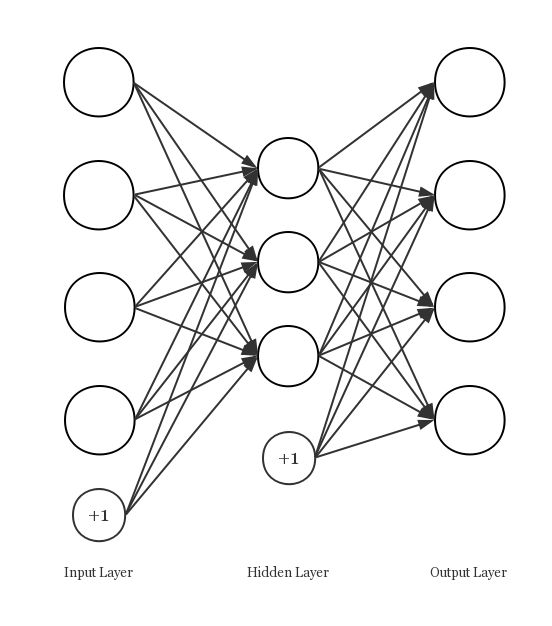
\includegraphics[width=0.45\textwidth]{pictures/autoencoder} %插入图片命令,格式为[配置]{图片路径}
    }
    \quad %空格
    \subfloat[]{
	\label{Fig:R2} % 子图2标签名
    	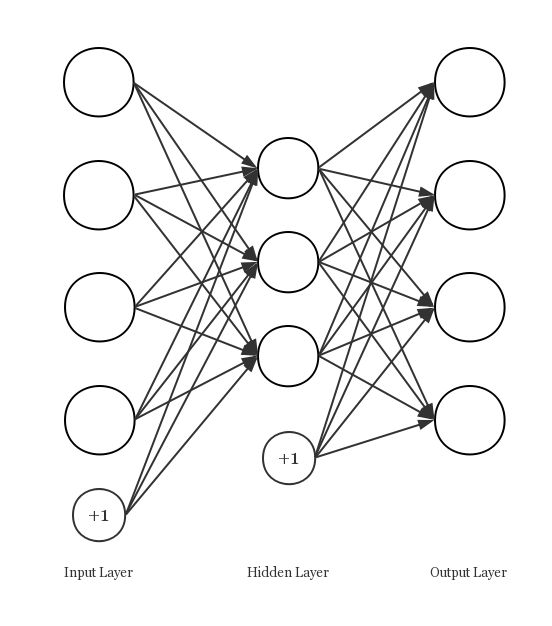
\includegraphics[width=0.45\textwidth]{pictures/autoencoder}
    }
    \caption{这是两个自编码器结构,我就是排一下子图的效果:\protect\subref{Fig:R1}左边的自编码器,\protect\subref{Fig:R2}右边的自编码器} %注意须使用\protect\subref{}进行标号引用
    \label{Fig:RecAccuracy} % 整个组图的标签名
\end{figure}

\section{公式与算法表示}

\subsection{例子:基于主成分分析}

\subsubsection{主成分分析算法}

下面对主成分分析进行介绍。

主成分分析是一种简单的机器学习算法,其功能可以从两方面解释:一方面可以认为它提供了一种压缩数据的方式,另一方面也可以认为它是一种学习数据表示的无监督学习算法。\cite{Goodfellow2016DeepLearning}
通过PCA,我们可以得到一个恰当的超平面及一个投影矩阵,通过投影矩阵,样本点将被投影在这一超平面上,且满足最大可分性(投影后样本点的方差最大化),直观上讲,也就是能尽可能分开。

对中心化后的样本点集$\bm{X}=\{\bm{x}_1,\bm{x}_2,\ldots,\bm{x}_i,\ldots,\bm{x}_m\}$(有$\sum_{i=1}^{m}\bm{x}_i = 0$),考虑将其最大可分地投影到新坐标系\ $\bm{W}= \{\bm{w}_1,\bm{w}_2,\ldots,\bm{w}_i,\ldots,\bm{w}_d\} $,其中$\bm{w}_i$是标准正交基向量,满足$\|\bm{w}_i\|_2 = 1$, $\bm{w}_i^T\bm{w}_j = 0$($i \not= j$)。假设我们需要$d^\prime$($d^\prime < d$)个主成分,那么样本点$\bm{x}_i$在低维坐标系中的投影是$\bm{z}_i = (z_{i1};z_{i2};\ldots;z_{id^\prime})$,其中$z_{ij} = \bm{w}_j^\mathrm{T}\bm{x}_i$,是$\bm{x}_i$在低维坐标系下第$j$维的坐标。
对整个样本集,投影后样本点的方差是
\begin{equation}
\begin{aligned}
    & \frac{1}{m}\sum_{i=1}^m \bm{z}_i^\mathrm{T}\bm{z}_i \\
= & \frac{1}{m}\sum_{i=1}^m (\bm{x}_i^\mathrm{T}\bm{W})^\mathrm{T}(\bm{x}_i^\mathrm{T}\bm{W}) \\
= & \frac{1}{m}\sum_{i=1}^m \bm{W}^\mathrm{T}\bm{x}_i\bm{x}_i^\mathrm{T}\bm{W} \\
= & \frac{1}{m} \bm{W}^\mathrm{T}\bm{X}\bm{X}^\mathrm{T}\bm{W} \\
\end{aligned}
\end{equation}

由于我们知道新坐标系$\bm{W}$的列向量是标准正交基向量,且样本点集$\bm{X}$已经过中心化,则PCA的优化目标可以写为
\begin{equation}
\label{PCA_goal}
\begin{aligned}
& \max_{\substack{\bm{W}}}  &  tr(\bm{W}^\mathrm{T}\bm{X}\bm{X}^ \mathrm{T}\bm{W}) \\
& \operatorname{ s.t. }  &  \bm{W}^\mathrm{T}\bm{W} = \bm{I} \\
\end{aligned}
\end{equation}

由于$\bm{X}\bm{X}^ \mathrm{ T }$是协方差矩阵,那么只需对它做特征值分解,即
\begin{equation}
\label{PCA_eigenvalue}
\bm{X}^ \mathrm{ T }\bm{X} = \bm{W}\bm{\Lambda}\bm{W}^ \mathrm{ T } \\
\end{equation}
其中$\bm{\Lambda}=diag(\bm{\lambda})$,$\bm{\lambda} = \{\lambda_1,\lambda_2,\ldots,\lambda_m\}$。

具体地,考虑到它是半正定矩阵的二次型,存在最大值,可对\eqref{PCA_goal}使用拉格朗日乘数法
\begin{equation}
\bm{X}\bm{X}^ \mathrm{ T }\bm{w}_i  = \lambda_i \bm{w}_i \\
\end{equation}

之后将求得的特征值降序排列,取前$d^\prime$个特征值对应的特征向量组成所需的投影矩阵$\bm{W}^\prime =(\bm{w}_1,\bm{w}_2,\ldots,\bm{w}_{d^\prime})$,即可得到PCA的解。PCA算法的描述如算法\ref{PCA_algorithm}所示。
\begin{algorithm} 
\floatname{algorithm}{算法}
\caption{主成分分析(PCA)} 
\label{PCA_algorithm}
\renewcommand{\algorithmicrequire}{\textbf{输入:}}
\renewcommand{\algorithmicensure}{\textbf{输出:}} 
\begin{algorithmic}[1] 
\Require 样本集$\bm{x}=\{\bm{x}_1,\bm{x}_2,\ldots,\bm{x}_i,\ldots,\bm{x}_m\}$,低维空间维数$d^\prime$ 
\Ensure 投影矩阵  $\bm{W}^\prime =(\bm{w}_1,\bm{w}_2,\ldots,\bm{w}_{d^\prime})$
\State 对所有样本中心化$\bm{x}_i \gets \bm{x}_i - \frac{1}{m}\sum_{i=1}^m \bm{x}_i$
\State  计算样本的协方差$\bm{X}\bm{X}^ \mathrm{T}$
\State 对协方差矩阵$\bm{X}\bm{X}^ \mathrm{T}$做特征值分解
\State 取最大的$d^\prime$个特征值所对应的特征向量$\bm{w}_1,\bm{w}_2,\ldots,\bm{w}_{d^\prime}$
\end{algorithmic}  
\end{algorithm}

\subsubsection{主成分分析可信度评估方法}
记待判定微博$\bm{w}_0$的经典特征向量为$\bm{f}^{c}_{0}$,它的发布者在$\bm{w_0}$前发布的$k$条微博为$\bm{W} = \bm{w}_1,\bm{w}_2,\ldots,\bm{w}_k$,这$k$条微博对应的经典特征向量集为$\bm{F}^{c}_{W} = \{ \bm{f}^{c}_{1},\bm{f}^{c}_{2},\ldots,\bm{f}^{c}_{k} \}$。令$label = 1$代表谣言,$label = 0$代表非谣言。算法的具体流程如算法\ref{PCA_model}所示。

\begin{algorithm} 
\floatname{algorithm}{算法}
\caption{基于PCA的信息可信度评估} 
\label{PCA_model}
\renewcommand{\algorithmicrequire}{\textbf{输入:}}
\renewcommand{\algorithmicensure}{\textbf{输出:}} 
	\begin{algorithmic}[1] 
	\Require $\bm{f}^{c}_{0}$,$\bm{F}^{c}_{W}$,保留主成分数$n$
	\Ensure 标签$label\in \{0,1\}$
	\State 对所有特征向量应用PCA,保留前$n$个主成分$\bm{o}^{c}_{i} \gets PCA(\bm{f}^{c}_{i}, n)$($i = 0,1,\ldots,k$)
	\State 计算$\bm{F}^{c}_{W}$中各向量的平均距离$\mu$和标准差$\sigma$
	\State 计算阈值$thr = {\mu} / {\sigma}$
	\If {$\min_{1<j\le k} \|\bm{o}^{c}_{0} - \bm{o}^{c}_{j} \|_2 > thr$}
		\State $ label \gets 1 $
	\Else
		\State $ label \gets 0 $
	\EndIf
	\end{algorithmic}
\end{algorithm}

\section{代码表示}
下面的代码\ref{plus}是用Python编写的加法函数。

\begin{lstlisting}[language=Python, caption=加法, label=plus, tabsize=2]  
def plus_func(a, b):
	return a + b
\end{lstlisting}  

\section{列表样式}

以下是使用圆点作为项目符号的列表样式。

\begin{itemize}
\item \textbf{第一章为基础模块示例},是的,就是本章。
\item \textbf{第二章为不存在},是的,其实它不存在。
\end{itemize}

以下是使用数字作为项目符号的列表样式。

\begin{enumerate}
\item \textbf{第一章为基础模块示例},是的,就是本章。
\item \textbf{第二章为不存在},是的,其实它不存在。
\end{enumerate}

以下是无项目符号(实际是可以自定义一些符号,但我懒得加了)的列表样式,它会顶格书写。

\begin{description}
\item \textbf{第一章为基础模块示例},是的,就是本章。
\item \textbf{第二章为不存在},是的,其实它不存在。
\end{description}

%%%%%%%%%%%%%%%%%%%%%%% Main Area ENDs Here %%%%%%%%%%%%%%%%%%%%%%%%
%\let\cleardoublepage=\cleardoublepagebak
% Reference
\clearpage\phantomsection\addcontentsline{toc}{chapter}{参考文献}
\bibliographystyle{buptbachelor}
\refbodyfont{\bibliography{ref}}

% Thanks to page
\clearpage\phantomsection\addcontentsline{toc}{chapter}{致\qquad{}谢}
\chapter*{致\qquad{}谢}
\normalsize\thankwords

% Appendix
\setcounter{figure}{0} 
\renewcommand{\thefigure}{~附-\arabic{figure}~}
\setcounter{equation}{0} 
\renewcommand{\theequation}{~附-\arabic{equation}~}
\setcounter{table}{0} 
\renewcommand{\thetable}{~附-\arabic{table}~}

\chapter*{附\qquad{}录}
\phantomsection\addcontentsline{toc}{chapter}{附\qquad{}录}

\phantomsection
\addcontentsline{toc}{section}{附录1\quad{}缩略语表}
\section*{附录1\quad{}缩略语表}

\begin{bupttable}{基于浏览者行为的特征}{crowdwisdom}
    \begin{tabular}{l|l|l}
		\hline \textbf{特征} & \textbf{描述} & \textbf{形式与理论范围}\\
		\hline 点赞量 & 微博的点赞数量 & 数值,$\mathbb{N}$ \\
		\hline 评论量 & 微博的评论数量 & 数值,$\mathbb{N}$ \\
		\hline 转发量 & 微博的转发数量 & 数值,$\mathbb{N}$ \\
		\hline
    \end{tabular}
\end{bupttable}
\buptfigure[width=0.7\textwidth]{pictures/autoencoder}{自编码器结构}{autoencoder}

\begin{equation}
\label{PCA_goal}
\begin{aligned}
\max_{\substack{\bm{W}}}  &  tr(\bm{W}^\mathrm{T}\bm{X}\bm{X}^ \mathrm{T}\bm{W})
\end{aligned}
\end{equation}

\phantomsection
\addcontentsline{toc}{section}{附录2\quad{}数学符号}
\section*{附录2\quad{}数学符号}
\begin{center}
	\begin{tabular}{ccc}
		\multicolumn{2}{c}{\textbf{数和数组}} \\
		\\
		$a$ & 标量(整数或实数)\\
		$\bm{a}$ & 向量\\
		$dim()$ & 向量的维数\\
		$\bm{A}$ & 矩阵\\
		$\bm{A}^\mathrm{T}$ & 矩阵$\textbf{A}$的转置\\
		$\bm{I}$ & 单位矩阵(维度依据上下文而定) \\
 		$diag(\bm{a})$ & 对角方阵,其中对角元素由向量$\bm{a}$确定 \\

	\end{tabular}
\end{center}

\newpage\backmatter
% Translation
\chapter*{外\quad{}文\quad{}译\quad{}文}
\vspace{8mm}

\thispagestyle{empty}

\begin{center}
\sihao\heiti{真假新闻的在线传播}

\xiaosihao\songti{Soroush Vosoughi, Deb Roy, Sinan Aral}

\xiaosihao\songti{麻省理工学院}
\end{center}

\songti{}
决策、合作、通信和市场领域的基础理论全都将对真实或准确度的概念化作为几乎一切人类努力的核心。然而,不论是真实信息还是虚假信息都会于在线媒体上迅速传播。定义什么是真、什么是假成了一种常见的政治策略,而不是基于一些各方同意的事实的争论。我们的经济也难免遭受虚假信息传播的影响。虚假流言会影响股价和大规模投资的动向,例如,在一条声称巴拉克·奥巴马在爆炸中受伤的推文发布后,股市市值蒸发了1300亿美元。的确,从自然灾害到恐怖袭击,我们对一切事情的反应都受到了扰乱。
新的社交网络技术在使信息的传播速度变快和规模变大的同时,也便利了不实信息(即不准确或有误导性的信息)的传播。然而,尽管我们对信息和新闻的获取越来越多地收到这些新技术的引导,但我们仍然对他们在虚假信息传播上的作用知之甚少。尽管媒体对假新闻传播的轶事分析给予了相当多的关注,但仍然几乎没有针对不实信息扩散或其发布源头的大规模实证调查。目前,虚假信息传播的研究仅仅局限于小的、局部的样本的分析上,而这些分析忽略了两个最重要的科学问题:真实信息和虚假信息的传播有什么不同?哪些人类判断中的因素可以解释这些不同?

% Translated Article
\thispagestyle{empty}
\begin{center}
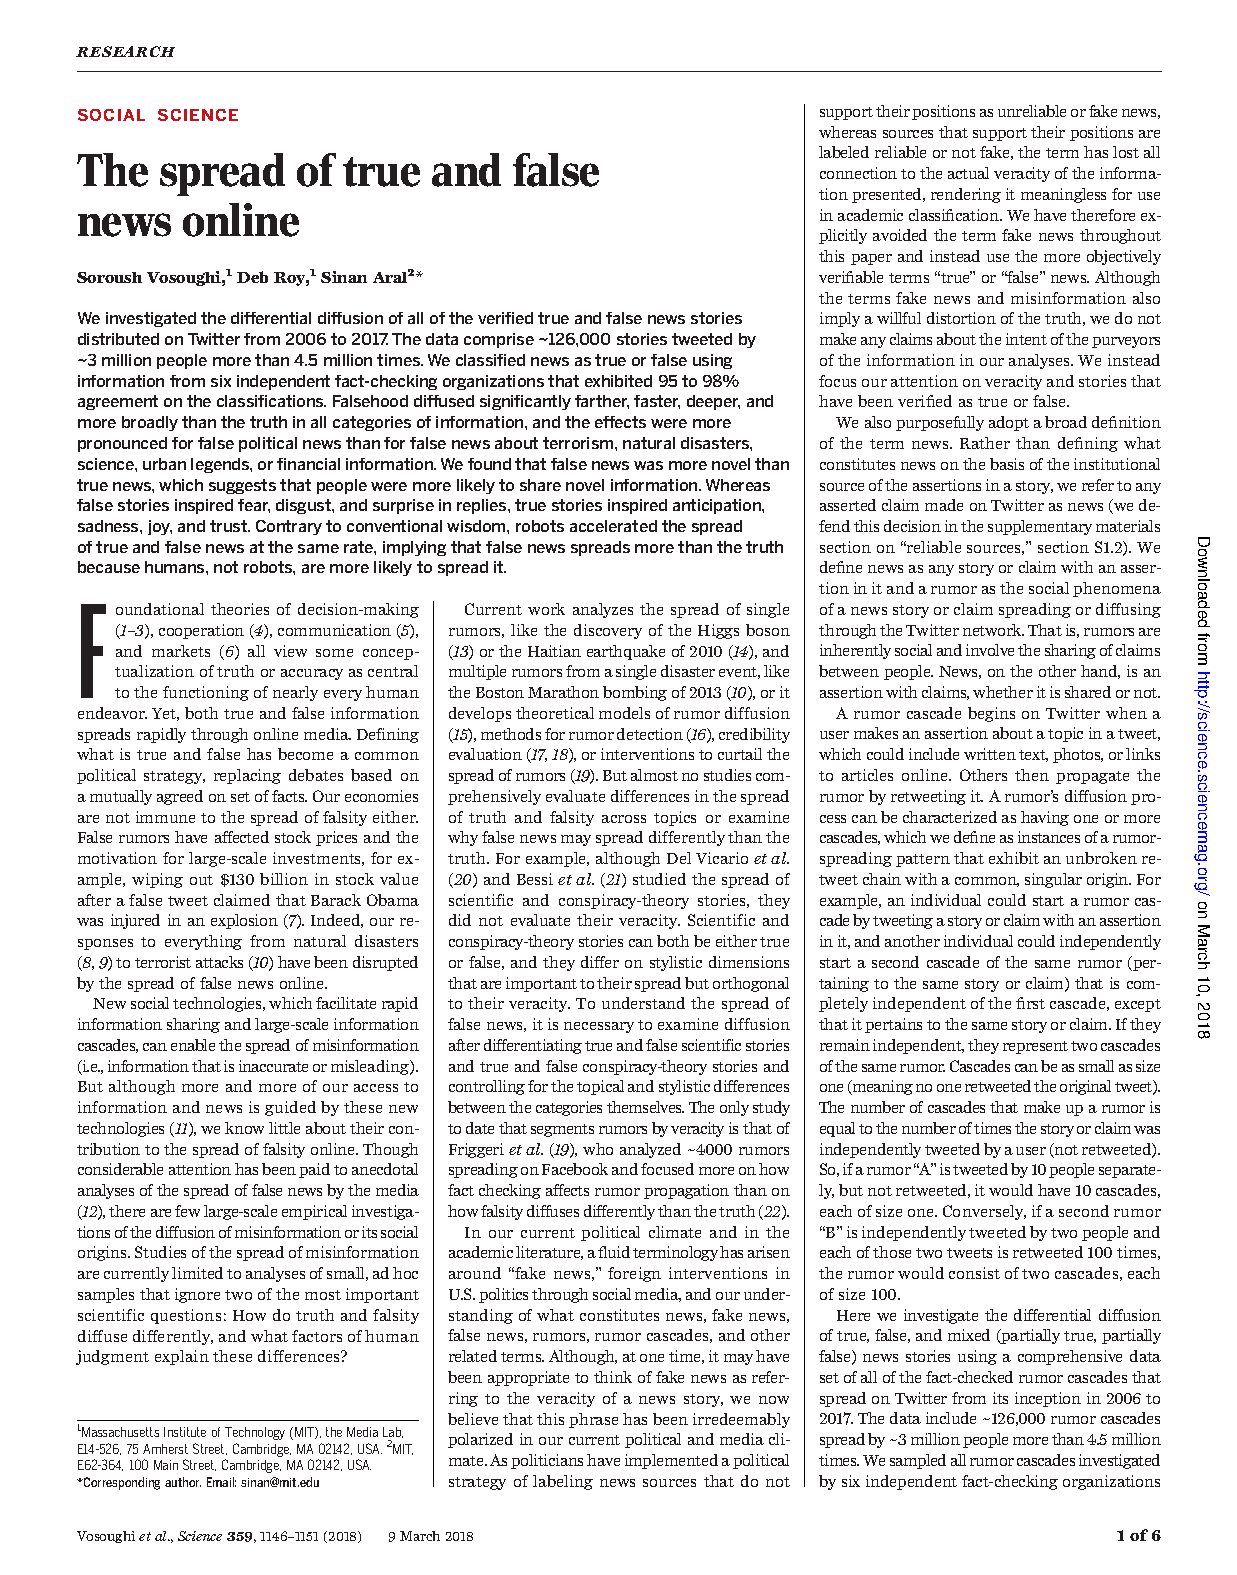
\includepdf[pages=1, scale=0.95, pagecommand=\heiti\sanhao{外\quad{}文\quad{}原\quad{}文}]{docs/translation.pdf}
\includepdf[pages=2-, scale=0.95, pagecommand={}]{docs/translation.pdf}
\end{center}

% 开题报告
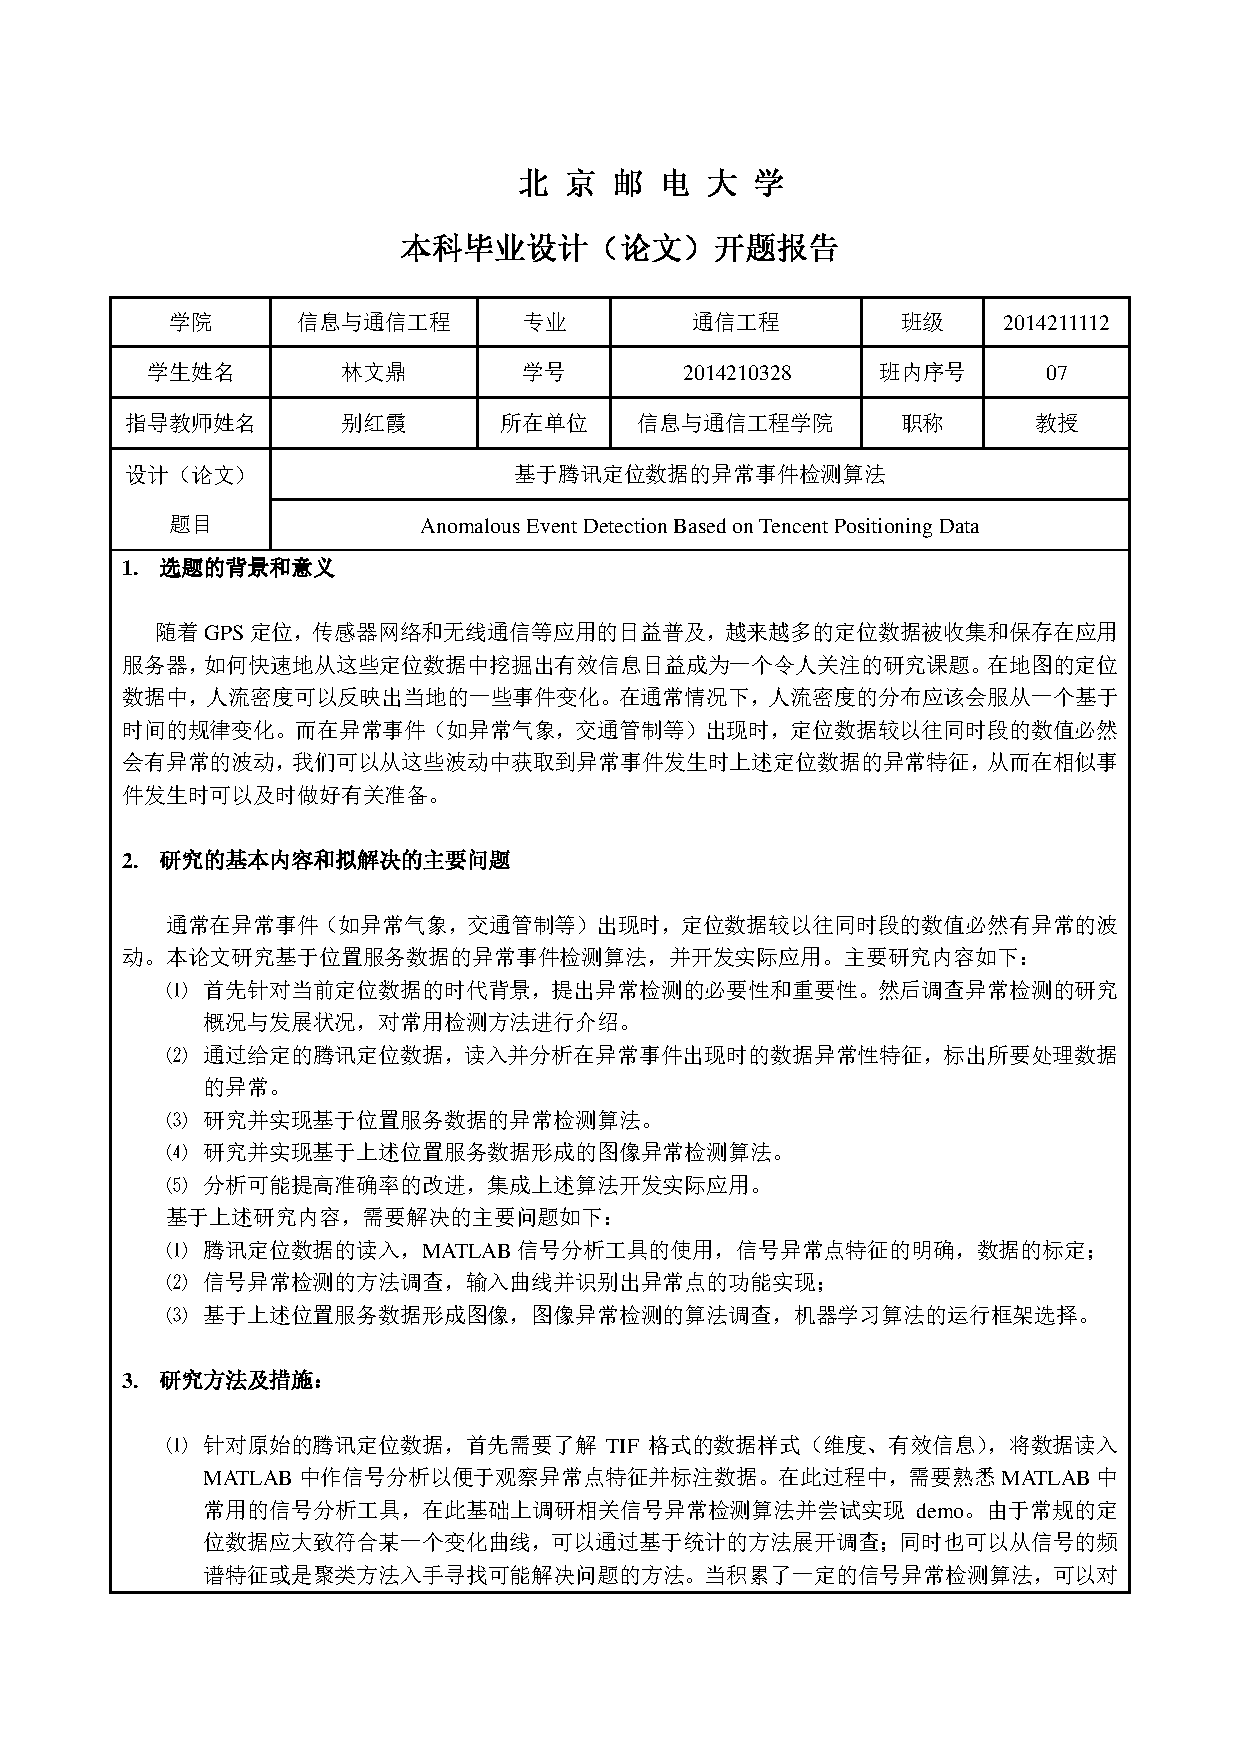
\includepdf[pages=-]{docs/openingReport.pdf} 


% 中期检查表
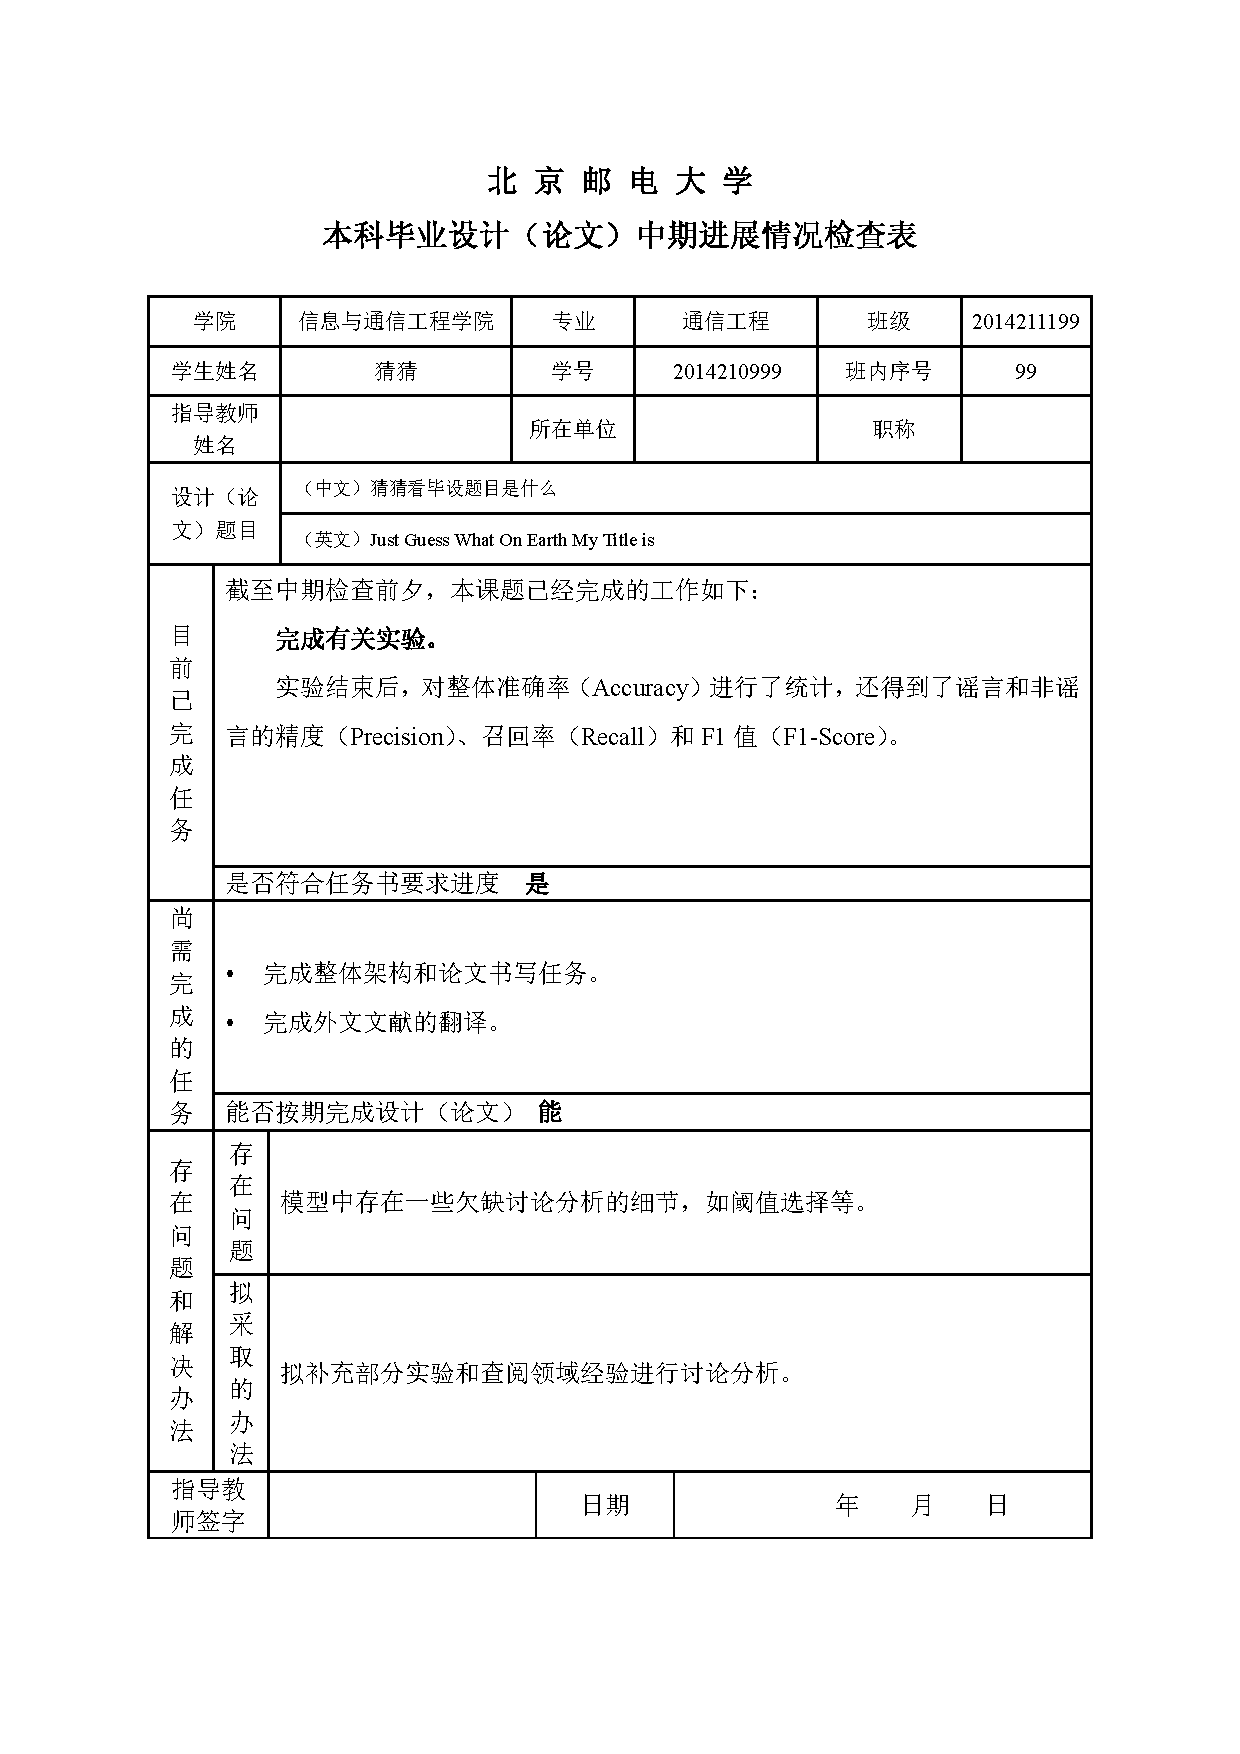
\includepdf[pages=-]{docs/interimReport.pdf} 


\end{document}
